\documentclass[tikz,border=6pt]{standalone}
\usepackage{amsmath,amssymb,mathtools,physics,bm,nicefrac,wasysym}
\usepackage{xcolor}

\definecolor{colone}{RGB}{180,60,60}
\definecolor{coltwo}{RGB}{60,110,180}
\definecolor{colthree}{RGB}{60,140,80}

\definecolor{accent}{HTML}{A13D2C}
\definecolor{accent2}{HTML}{2B5F6B}
\definecolor{muted}{HTML}{5A564F}
\definecolor{panel}{HTML}{F8F6F0}
\definecolor{linecol}{HTML}{D8D2C4}
\definecolor{ink}{HTML}{1E1C1A}
\definecolor{astroblue}{HTML}{1B4F72}
\definecolor{astrodark}{HTML}{17202A}
\definecolor{sunyellow}{HTML}{E8A33D}

\usetikzlibrary{calc,arrows.meta,positioning,decorations.pathreplacing,decorations.markings,angles,quotes,shapes.geometric}
\usepackage{tikz-3dplot}

\newcommand{\vecr}{\vec r}
\newcommand{\vecL}{\vec L}
\newcommand{\vecA}{\vec A}
\newcommand{\vecf}{\vec f}
\newcommand{\vecF}{\vec F}
\newcommand{\vecp}{\vec p}
\newcommand{\avg}[1]{\left\langle #1\right\rangle}
\newcommand{\vecx}{\vec x}
\newcommand{\hatn}{\hat n}
\newcommand{\rhat}{\hat r}
\newcommand{\phihat}{\hat\phi}
\newcommand{\thetahat}{\hat\theta}
\newcommand{\note}[1]{\textcolor{blue!60!black}{\textit{[#1]}}}

% Astronomical acronyms
\newcommand{\LST}{\mathrm{LST}}
\newcommand{\GST}{\mathrm{GST}}
\newcommand{\GMST}{\mathrm{GMST}}
\newcommand{\GAST}{\mathrm{GAST}}
\newcommand{\LMST}{\mathrm{LMST}}
\newcommand{\LAST}{\mathrm{LAST}}
\newcommand{\UT}{\mathrm{UT}}
\newcommand{\UTC}{\mathrm{UTC}}
\newcommand{\TAI}{\mathrm{TAI}}
\newcommand{\TT}{\mathrm{TT}}
\newcommand{\TDB}{\mathrm{TDB}}
\newcommand{\JD}{\mathrm{JD}}
\newcommand{\MJD}{\mathrm{MJD}}
\newcommand{\EoT}{\mathrm{EoT}}
\newcommand{\SNR}{\mathrm{SNR}}
\newcommand{\RON}{\mathrm{RON}}

% Helper commands for specific diagrams
\newcommand{\midlinelabel}[3]{
    \node (midlabel) at ($ (#1)!.5!(#2) $) {#3};
    \draw[stealth-] (#1) --  (midlabel);
    \draw[-stealth] (midlabel) -- (#2);
}
\newcommand{\midlinelabell}[3]{
    \node[fill = white, inner sep = 0.2pt, outer sep=3pt] (midlabel) at ($ (#1)!.5!(#2) $) {#3};
    \draw[stealth-] (#1) --  (midlabel);
    \draw[-stealth] (midlabel) -- (#2);
}
\newcommand{\midlinelabelll}[3]{
    \node[fill = white, inner sep = 0.2pt, outer sep=3pt,scale=0.6] (midlabel) at ($ (#1)!.5!(#2) $) {#3};
    \draw[stealth-] (#1) --  (midlabel);
    \draw[-stealth] (midlabel) -- (#2);
}



\begin{document}
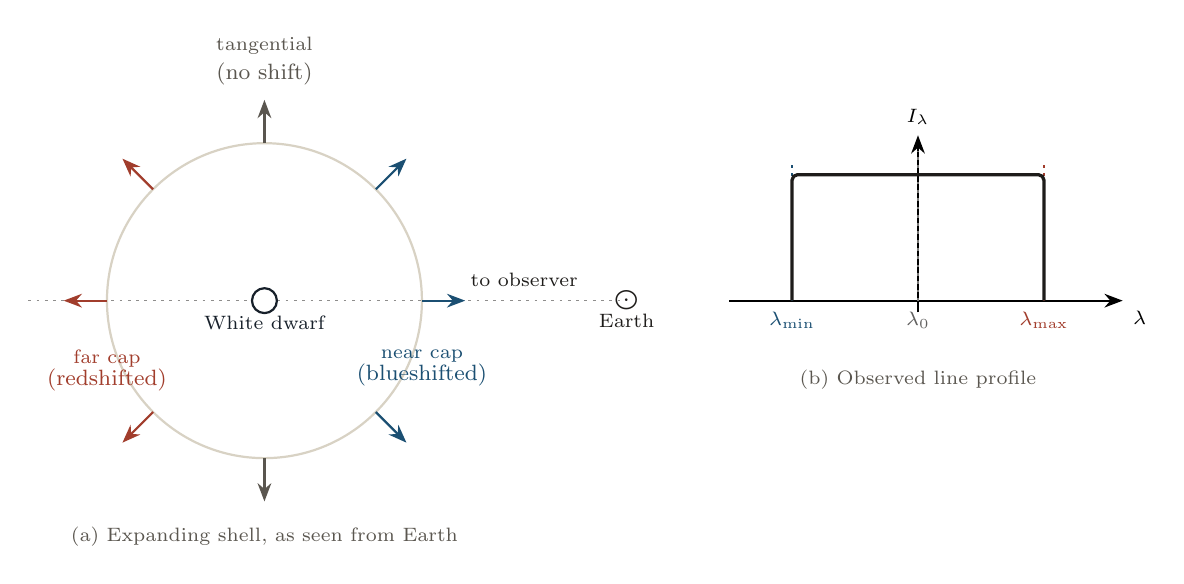
\begin{tikzpicture}[>=Stealth, scale=1.0, font=\scriptsize]

		% ================= Panel (a): expanding shell geometry =================
		\coordinate (C) at (0,0); % central white dwarf

		% the expanding shell
		\draw[linecol, thick] (C) circle (2.0);

		% line of sight axis
		\draw[ink!50, dash pattern=on 1pt off 2pt, thin] (-3.0,0) -- (4.6,0);

		% radial velocity vectors around the shell, color-coded by line-of-sight sense
		\foreach \phi in {0,45,90,135,180,225,270,315}{
			\coordinate (P) at (\phi:2.0);
			\coordinate (Q) at (\phi:2.55);
			\pgfmathsetmacro{\c}{cos(\phi)}
			\ifdim \c pt > 0.35pt
				\draw[astroblue, thick, ->] (P) -- (Q);
			\else
				\ifdim \c pt < -0.35pt
					\draw[accent, thick, ->] (P) -- (Q);
				\else
					\draw[muted, thick, ->] (P) -- (Q);
				\fi
			\fi
		}

		% central white dwarf
		\fill[white] (C) circle (4.5pt);
		\draw[astrodark, thick] (C) circle (4.5pt);
		\node[astrodark, below=2pt] at (C) {White dwarf};

		% near cap (facing observer) and far cap labels
		\node[astroblue, below, align=center] at (2.0,-0.5) {near cap\\\footnotesize(blueshifted)};
		\node[accent, below, align=center] at (-2.0,-0.5) {far cap\\\footnotesize(redshifted)};
		\node[muted, above=2pt] at (0,2.55) {\shortstack{tangential\\\footnotesize(no shift)}};

		% observer
		\node[ink] at (4.6,0) {$\bigodot$};
		\node[ink, below] at (4.6,-0.05) {Earth};
		\node[ink, above, font=\scriptsize] at (3.3,0.05) {to observer};

		\node[muted] at (0,-3.0) {(a) Expanding shell, as seen from Earth};

		% ================= Panel (b): resulting line profile =================
		\begin{scope}[xshift=8.3cm]
			\draw[->, thick] (-2.4,0) -- (2.6,0) node[below right] {$\lambda$};
			\draw[->, thick] (0,-0.15) -- (0,2.1) node[above] {$I_\lambda$};

			% rest wavelength
			\draw[ink!60, dash pattern=on 1pt off 2pt, thin] (0,0) -- (0,1.9);
			\node[ink!70, below] at (0,-0.02) {$\lambda_0$};

			% blue / red extremes
			\draw[astroblue, dash pattern=on 1pt off 2pt, thin] (-1.6,0) -- (-1.6,1.75);
			\draw[accent, dash pattern=on 1pt off 2pt, thin] (1.6,0) -- (1.6,1.75);
			\node[astroblue, below] at (-1.6,-0.02) {$\lambda_{\min}$};
			\node[accent, below] at (1.6,-0.02) {$\lambda_{\max}$};

			% flat-topped emission profile
			\draw[very thick, ink, rounded corners=2pt]
				(-1.6,0) -- (-1.6,1.6) -- (1.6,1.6) -- (1.6,0);

			\node[muted] at (0,-1.0) {(b) Observed line profile};
		\end{scope}

	\end{tikzpicture}
\end{document}
